\usetikzlibrary{decorations.markings}

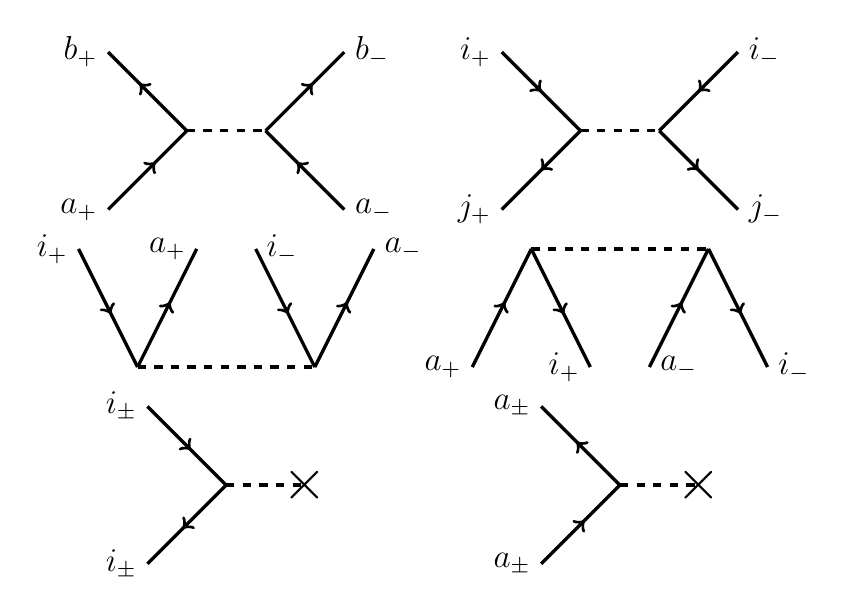
\begin{tikzpicture}[
        cross/.style={
            cross out,
            draw=black,
            minimum size=2*(#1-\pgflinewidth),
            inner sep=0pt,
            outer sep=0pt
        }, %default radius will be 1pt.
        cross/.default={1pt}
    ]

    \begin{scope}[very thick,decoration={
                markings,
                mark=at position 0.6 with {\arrow{>}}
            }
        ]
        \coordinate (upleft) at (0, 2) {};
        \coordinate (downleft) at (0, 0) {};
        \coordinate (midleft) at (1, 1) {};
        \coordinate (midright) at (2, 1) {};
        \coordinate (upright) at (3, 2) {};
        \coordinate (downright) at (3, 0) {};

        \draw[postaction={decorate}]   (downleft) node[left] {\large$a_+$} -- (midleft);
        \draw[postaction={decorate}]   (midleft) -- (upleft) node[left] {\large$b_+$};
        \draw[dashed] (midleft) -- (midright);
        \draw[postaction={decorate}]   (downright) node[right] {\large$a_-$} -- (midright) ;
        \draw[postaction={decorate}]   (midright) -- (upright) node[right] {\large$b_-$};

    \end{scope}

    \begin{scope}[xshift=5cm,very thick,decoration={
                markings,
                mark=at position 0.5 with {\arrow{>}}
            }
        ]
        \coordinate (upleft) at (0, 2) {};
        \coordinate (downleft) at (0, 0) {};
        \coordinate (midleft) at (1, 1) {};
        \coordinate (midright) at (2, 1) {};
        \coordinate (upright) at (3, 2) {};
        \coordinate (downright) at (3, 0) {};

        \draw[postaction={decorate}] (upleft) node[left] {\large$i_+$} -- (midleft);
        \draw[postaction={decorate}] (midleft) -- (downleft) node[left] {\large$j_+$};
        \draw[dashed] (midleft) -- (midright);
        \draw[postaction={decorate}] (upright) node[right] {\large$i_-$} -- (midright);
        \draw[postaction={decorate}] (midright) -- (downright) node[right] {\large$j_-$};
    \end{scope}

    \begin{scope}[xshift=-0.375cm,yshift=-3cm,very thick,decoration={
                markings,
                mark=at position 0.55 with {\arrow{>}}
            }
        ]
        \coordinate (leftin) at (0, 2.5) {};
        \coordinate (lefout) at (1.5, 2.5) {};
        \coordinate (midleft) at (.75, 1) {};
        \coordinate (midright) at (3, 1) {};
        \coordinate (rightin) at (2.25, 2.5) {};
        \coordinate (rightout) at (3.75, 2.5) {};

        \draw[postaction={decorate}] (leftin) node[left] {\large$i_+$} -- (midleft);
        \draw[postaction={decorate}] (midleft) -- (lefout) node[left] {\large$a_+$};
        \draw[dashed] (midleft) -- (midright);
        \draw[postaction={decorate}] (rightin) node[right] {\large$i_-$} -- (midright);
        \draw[postaction={decorate}] (midright) -- (rightout) node[right] {\large$a_-$};
    \end{scope}

    \begin{scope}[xshift=5cm-0.375cm,yshift=-3cm,very thick,decoration={
                markings,
                mark=at position 0.55 with {\arrow{>}}
            }
        ]
        \coordinate (leftin) at (0, 1) {};
        \coordinate (lefout) at (1.5, 1) {};
        \coordinate (midleft) at (.75, 2.5) {};
        \coordinate (midright) at (3, 2.5) {};
        \coordinate (rightin) at (2.25, 1) {};
        \coordinate (rightout) at (3.75, 1) {};

        \draw[postaction={decorate}] (leftin) node[left] {\large$a_+$} -- (midleft);
        \draw[postaction={decorate}] (midleft) -- (lefout) node[left] {\large$i_+$};
        \draw[dashed] (midleft) -- (midright);
        \draw[postaction={decorate}] (rightin) node[right] {\large$a_-$} -- (midright);
        \draw[postaction={decorate}] (midright) -- (rightout) node[right] {\large$i_-$};
    \end{scope}

    \begin{scope}[xshift=0.5cm,yshift=-4.5cm,very thick,decoration={
                markings,
                mark=at position 0.55 with {\arrow{>}}
            }
        ]
        \coordinate (leftin) at (0, 2) {};
        \coordinate (leftout) at (0, 0) {};
        \coordinate (midleft) at (1, 1) {};
        \coordinate (midright) at (2, 1) {};

        \draw[postaction={decorate}] (leftin) node[left] {\large$i_{\pm}$} -- (midleft);
        \draw[postaction={decorate}] (midleft) -- (leftout) node[left] {\large$i_{\pm}$};
        \draw[dashed] (midleft) -- (midright);

        \node at (midright) {\huge$\times$};

    \end{scope}

    \begin{scope}[xshift=5.5cm,yshift=-4.5cm,very thick,decoration={
                markings,
                mark=at position 0.55 with {\arrow{>}}
            }
        ]
        \coordinate (leftin) at (0, 0) {};
        \coordinate (leftout) at (0, 2) {};
        \coordinate (midleft) at (1, 1) {};
        \coordinate (midright) at (2, 1) {};

        \draw[postaction={decorate}] (leftin) node[left] {\large$a_{\pm}$} -- (midleft);
        \draw[postaction={decorate}] (midleft) -- (leftout) node[left] {\large$a_{\pm}$};
        \draw[dashed] (midleft) -- (midright);

        \node at (midright) {\huge$\times$};

    \end{scope}

    % \begin{scope}[xshift=5cm,very thick,decoration={
    %             markings,
    %             mark=at position 0.55 with {\arrow{>}}
    %         }
    %     ]
    %     \node at (-1, 1) {\huge$+$};
    %     \coordinate (upleft) at (0, 2) {};
    %     \coordinate (downleft) at (0, 0) {};
    %     \coordinate (upright) at (1, 2) {};
    %     \coordinate (downright) at (1, 0) {};

    %     \draw[postaction={decorate}]   (downleft) node[below] {\large$p_+$} -- (upleft) node[above] {\large$p_+$};
    %     \draw[postaction={decorate}]   (downright) node[below] {\large$p_-$} -- (upright) node[above] {\large$p_-$};
    % \end{scope}
\end{tikzpicture}

% \end{document}
